\documentclass[../main.tex]{subfiles}
\graphicspath{
    {"../img/"}
    {"img/"}
}

\begin{document}
Jeżeli $f$ - holomorficzna na $R(z_0, 0, r_2)$, to
\[
    f(z) = \sum_{n = 0}^{\infty} a_n (z-z_0)^n
\]
Mamy
\[
    a_n = \frac{1}{2 \pi i} \int\limits_{\partial K(z_0, r)} \frac{f(\xi)}{(\xi - z_0)^{n+1}},\quad r_1 < r < r_2
.\]
ale możemy zauważyć, że
\[
    a_n = \frac{f^{(n)}(z_0)}{n!}
\]
\begin{przyklad}
    Policzyć
    \[
        I = \int\limits_{\partial K(i, 1)} \frac{\cos (z)}{(1+z^2)^2} dz
    .\]
Zauważmy, że
    \[
        \frac{\cos(z)}{(1+z^2)^2} = \frac{\cos(z)}{(1+iz)^2(1-iz)^2}
    .\]
    Niech $f(z) = \frac{\cos(z)}{(1 - iz)^2}$, $f$ - holomorficzna na $K(i,1)$. W związku z tym piszemy
    \[
        I = \int\limits_{\partial K(i,1)} \frac{f(z)}{(1+iz)^2}dz = \frac{1}{(i)^2} \int\limits_{\partial K(i,1)} \frac{f(z) dz}{(z-i)^2} = (i)^2 \cdot 2\pi i \left. f'(z) \right|_{z = i}
    .\]
\end{przyklad}
\subsection{Przedłużenie analityczne (oho)}
Mieliśmy np. $\sin(x)$ dla $x\in \mathbb{R}$ i pytanie skąd my wiemy, że $\sin(z) = \frac{1}{2i} \left(e^{iz} - e^{-iz}\right)$, dla $z \in \mathbb{C}$

\begin{tw}
    Niech $\mathcal{O}\subset\mathbb{C}$, $f$ - holomorficzna na $\mathcal{O}$,\\
    $z_n\in\mathcal{O}$ - ciąg z $\mathcal{O}$ taki, że $z_n \underset{n\to \infty}{\longrightarrow}z_0 \underset{n\in \mathbb{N}}{\forall} f(z_n) = 0$.\\
    Wówczas
    \[
        \underset{r > 0}{\exists}\quad \underset{z\in K(z_0, r)}{\forall} \quad f(z) = 0
    .\]
\end{tw}
\begin{proof}
    przez sprzeczność ($\lnot(p\implies q) \iff (p \land \lnot q)$).\\
    Załóżmy, że $\underset{z\in K(z_0, r)}{\exists}\quad f(z) \neq 0$ i założenia twierdzenia są spełnione. Skoro $f$ - holomorficzna na $\mathcal{O}$, to możemy zapisać, że
    \[
        f(z) = \sum_{n = 0}^\infty \frac{f^{(n)}(z_0)}{n!} (z-z_0)^n
    \]
    i wiemy, że $f(z) \neq 0$, czyli $\exists k$ takie, że
    \begin{equation}
        \label{eqn: w12-1}
        \frac{f^{(k)}(z_0)}{k!} \neq 0 \tag{$\star$}
    .\end{equation}
    Weźmy najmniejszy indeks, dla którego \eqref{eqn: w12-1} jest prawdziwe. Oznaczmy ten indeks przez $j$. Oznacza to, że
    \[
        f(z) = (z - z_0)^j\left( \frac{f^{(j)}(z_0)}{j!} + \frac{f^{(j+1)}(z_0)}{(j+1)!} (z-z_0) + \dots\right)
    .\]
Czyli
    \[
        f(z) = (z-z_0)^j g(z),\quad f(z) \neq 0
    ,\]
czyli $g(z) \neq 0$. Skoro $f$ - holomorficzna, to $g(z)$ też jest holomorficzna na $\mathcal{O}$, czyli między innymi $g(z)$ jest ciągła na $\mathcal{O}$. Ale wiemy, że $f(z_n) = 0$, czyli $g(z_n) = 0$ i $g$ - ciągła na $\mathcal{O}$. Oznacza to, że
    \[
        0 = g(z_n) \underset{z_n\to z_0}{\longrightarrow} g(z_0) = 0
    \]
    i sprzeczność, bo $g(z_n)$ jest ciągiem samych zer, a $g(z_0) \neq 0$, bo
    \[
        \frac{f^{(j)}(z_j)}{j!} \neq 0
    .\]
\end{proof}
\textbf{Obserwacja: } Weźmy funkcję
\[
    f(x) = x^2 \sin\left(\frac{1}{x}\right),\quad x\in \mathbb{R}
.\]
Widzimy, że dla ciągu $a_n \to 0$,
\[
    f(a_n) \longrightarrow 0
\]
i $f(x) \neq 0,\quad x\neq a_n$
\begin{figure}[h]
    \center
    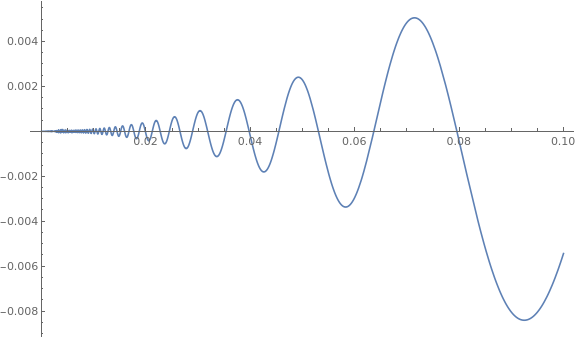
\includegraphics[width=.5\textwidth]{fig12-1}
    \caption{$f(x)$}
\end{figure}

\begin{tw}
    Niech $f(z),g(z)$ - holomorficzne na $\mathcal{O}$,
    \[
        \underset{h \in \mathbb{N}}{\forall} f(z_n) = g(z_n)
    \]
    a ciąg $z_n\to z_0$. Wówczas
    \[
        f(z) = g(z) \underset{z\in \mathcal{O}}{\forall}
    .\]
\end{tw}
\begin{proof}
    Niech
    \[
        h(z) = f(z) - g(z)
    .\]
Wówczas $h(z_n) = 0$ i $z_n\to z_0$. Skoro $h(z)$ - holomorficzna, to znaczy, że
    \[
        f(z) = \sum_{n = 0}^{\infty} a_n (z-z_0)^n
    \]
    \[
        g(z) = \sum_{n = 0}^{\infty} b_n (z-z_0)^n
    \]
    oraz
    \[
        h(z) = \sum_{n = 0}^{\infty} (a_n - b_n) (z-z_0)^n
    \]
    i dowodzimy tak jak wcześniej.
\end{proof}
\begin{przyklad}
    \[
        f(z) = 1 + z + z^2 + z^3 + \dots,\quad |z| < 1
    \]
    \[
        g(z) = 1 + \left(\frac{z+1}{2}\right) + \left(\frac{z+1}{2}\right)^2 + \dots\quad \left| \frac{z+1}{2} \right| < 1
    \]
\begin{figure}[h]
    \center
    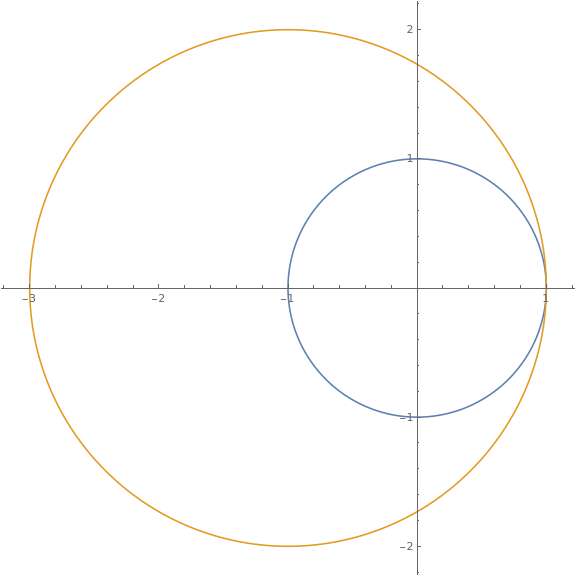
\includegraphics[width=.3\textwidth]{fig12-2}
    \caption{$f$ i $g$}
\end{figure}
\end{przyklad}
\begin{definicja}
    Niech $f$ - holomorficzna na $U_1$ i $g$ - holomorficzna na $U_2$ i
    \[
        \underset{z_0}{\exists} \in U_1\cap U_2 \implies \exists r: K(z_0,r) \subset U_1\cap U_2
    \]
    oraz
    \[
        \underset{z\in U_1\cap U_2}{\forall}\quad f(z) = g(z)
    .\]
Mówimy wówczas, że $f$ jest przedłużeniem holomorficznym (analitycznym funkcji $g$.
\end{definicja}
\begin{przyklad}
    Co się stanie jak będziemy przedłużać aż do kółka

    \[
        ln(z) = (z - 1) - \frac{1}{z}(z-1)^2 + \dots
    \]
    \[
        ln(re^{i\varphi}) = ln(r) + ln\left(e^{i\varphi}\right) = ln(r) + i\varphi
    \]
\end{przyklad}
\subsubsection{Punkty osobliwe}
\begin{definicja}
    Punkt w którym $f(z)$ nie jest holomorficzna nazywamy punktem osobliwym.
\end{definicja}
\begin{definicja}
    Niech $f(z)$ - taka, że
    \[
        f(z) = \varphi(z) + \frac{B_1}{z - a} + \frac{B_2}{(z - a)^2} + \dots + \frac{B_N}{(z-a)^N}
    \]
    i $\varphi(z)$ - holomorficzna na $\mathcal{O}$ i $f(z)$ - holomorficzna na $\mathcal{O} - \{a\}$.

    O takiej funkcji powiemy, że ma w punkcie $a$ biegun rzędu $N$.
\end{definicja}
\textbf{Pytanie: } czy $f$ może nie być holomorficzna np. na krzywej $\gamma \subset \mathbb{C}$?\\
\textbf{Odpowiedź: } gdyby $f$ nie była holomorficzna na $\gamma \subset \mathbb{C}$, to
\[
    g(z) = \frac{1}{f(z)} = 0,\quad \forall z\in \gamma
,\]
a to oznacza, że $g(z) \equiv 0$ także dla $z\not\in \gamma$.
\end{document}
